\documentclass[a4paper,12pt]{article}

\usepackage[francais]{babel}
\usepackage[utf8]{inputenc}
\usepackage[official]{eurosym}
\usepackage{hyperref}
\usepackage{verbatim}
\usepackage{graphicx}

%opening
\title{Développement d'un module NetFilter de filtrage applicatif\\INF 358}
\author{Stéphane \textsc{Jacob} - John \textsc{Whitbeck} - Vincent \textsc{Zanotti}}
\date{15 mai 2008}

\begin{document}

\maketitle
%\newpage

\section*{Introduction}
L'objectif du projet était de développer un module \verb+netfilter+ pour réaliser du filtrage applicatif. Nous avions le choix entre deux angles d'attaques possibles : réaliser un module noyau pour \verb+netfilter+, ou bien réaliser une extension de \verb+netfilter+ en userspace, ce qui est d'ailleurs la stratégie employée par la future version de \verb+l7-filter+).

Nous avons choisi la solution userspace, que nous croyons clairement préférable ; elle est en particulier plus simple à développer (pas besoin de redémarrer le noyau pour chaque test échoué), elle est plus fiable (un crash du démon userspace ne fait pas paniquer le noyau), et elle permet enfin d'utiliser toutes les librairies existantes, en particulier les librairies d'expressions régulières standard, ce que ne permet pas un module noyau.\\

Compte tenu des similarités entre les deux projets, nous nous sommes inspirés de \verb+l7-filter-userspace+ \cite{RW}.

\newpage

\section{Présentation du projet}
L'objectif du projet, tel que défini par le sujet, était la réalisation d'une extension
pour \verb+netfilter+, afin de permettre un filtrage applicatif (en particulier un filtrage
pour les protocoles \verb+http+ et \verb+ftp+).

L'intérêt du projet est de pouvoir différencier différents types de connexion \verb+http+ ou \verb+ftp+,
pour permettre, entre autres, de les interdire, ou de limiter leur débit. Par exemple, l'extension
devrait permettre de repérer \og les requêtes de type \verb+GET+ sur des fichiers PDF en http \fg{}.

L'extension devrait donc permettre une utilisation du type :
\begin{itemize}
\item \verb+iptables -A FORWARD -p tcp -m webfilter --function get+\\ \verb+--urlsizemax 255 -j ACCEPT+ : le module \og webfilter \fg{} n'autorise que la fonction \verb+GET+ avec une URL de taille max 255 ;
\item \verb+iptables -A FORWARD -p tcp -m ftpfilter --function get+\\
\verb+--filetype pdf -j ACCEPT+\\
\verb+iptables -A FORWARD -p tcp -m ftpfilter --function list+\\
\verb+--filetype pdf -j ACCEPT+ : le module \og webfilter \fg{} n'autorise que les fonctions \verb+LIST+ et \verb+GET+ sur les fichiers PDF.
\end{itemize}

La possibilité de journaliser les évènements est aussi primordiale. En effet, il est indispensable que des évènements puissent être remontés en fonction des critères de filtrage. La cause du rejet d'une requête doit donc être spécifiée, par exemple, \og URL de taille $>$ 255 \fg{}.

\newpage

\section{Fonctionnement de Netfilter et possibilités offertes}
\section<presentation>[NetFilter]{Fonctionnement de NetFilter}
  \begin{frame}
    \frametitle{Architecture G�n�rale}
    \begin{figure}
      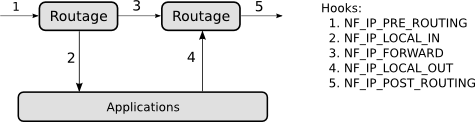
\includegraphics[scale=0.7]{pictures/netfilter.png}
    \end{figure}
  \end{frame}

  \begin{frame}
    \frametitle{Iptables: Principes}
    Fonctions: Regrouper en tables des r�gles de filtrage et de
    modification de paquets IP.

    \begin{center}
      \begin{tabular}{|l|l|}
	\hline
	\textbf{Table} & \textbf{Hooks} \\
	\hline
	filter & INPUT, OUTPUT, FORWARD \\
	\hline
	nat & PREROUTING, POSTROUTING \\
	\hline
	mangle & Toutes \\
	\hline
      \end{tabular}
    \end{center}

  \end{frame}

  \begin{frame}
    \frametitle{Iptables: Exemples}
    \begin{itemize}
    \item Filter: \\ 
      {\tt\scriptsize iptables -t filter -A INPUT -p tcp --dport 80 -j DROP}
    \item Nat: \\
      {\tt\scriptsize iptables -t nat -A POSTROUTING -d ! 192.168.0.0/24 -j
      SNAT --to-source 81.57.230.21}
    \item Mangle: \\
      {\tt\scriptsize iptables -t mangle -A POSTROUTING -p udp --dport 53 -j TOS --set-tos 16}
    \end{itemize}
  \end{frame}

  \begin{frame}
    \frametitle{Conntrack}
    Principe: 
    \begin{itemize}
    \item Regrouper les paquets en flux � partir des triplets (IP
    source, port source, port destination)
    \item Associer � chaque flux un �tat: NEW, ESTABLISHED, RELATED
    \end{itemize}
  \end{frame}

  \begin{frame}
    \frametitle{Extension de NetFilter}
    Plusieurs niveaux:
    \begin{itemize}
    \item Module noyau qui se branche directement sur un hook
    netfilter avec une extension iptables correspondante
    \item Application userspace. On utilise la cible \textrm{NFQUEUE}
    qui d�place un paquet de la m�moire noyau vers une file dans la
    m�moire userspace. Les paquets peuvent alors �tre trait�s par une
    application locale avant d'�tre reinject�s dans NetFilter.
    \end{itemize}
  \end{frame}


  \begin{frame}
    \frametitle{Notre choix}
    Application Userspace car:
    \begin{itemize}
    \item D�veloppement simplifi� et acc�s � des librairies
    puissantes (notamment pour la gestion d'expressions r�guli�res).
    \item Pas de plantage syst�me en cas de plantage de l'application
    \item Minimisation de l'impact d'une faille de s�curit� �ventuelle.
    \end{itemize}
    Mais: 
    \begin{itemize}
    \item Perte de performances due � la copie de la totalit� des
    paquets IP concern�s de la m�moire noyau vers la m�moire userspace
    et vice-versa.
    \end{itemize}
  \end{frame}

  \begin{frame}
    \frametitle{Principe g�n�ral de notre solution}
    \begin{figure}
      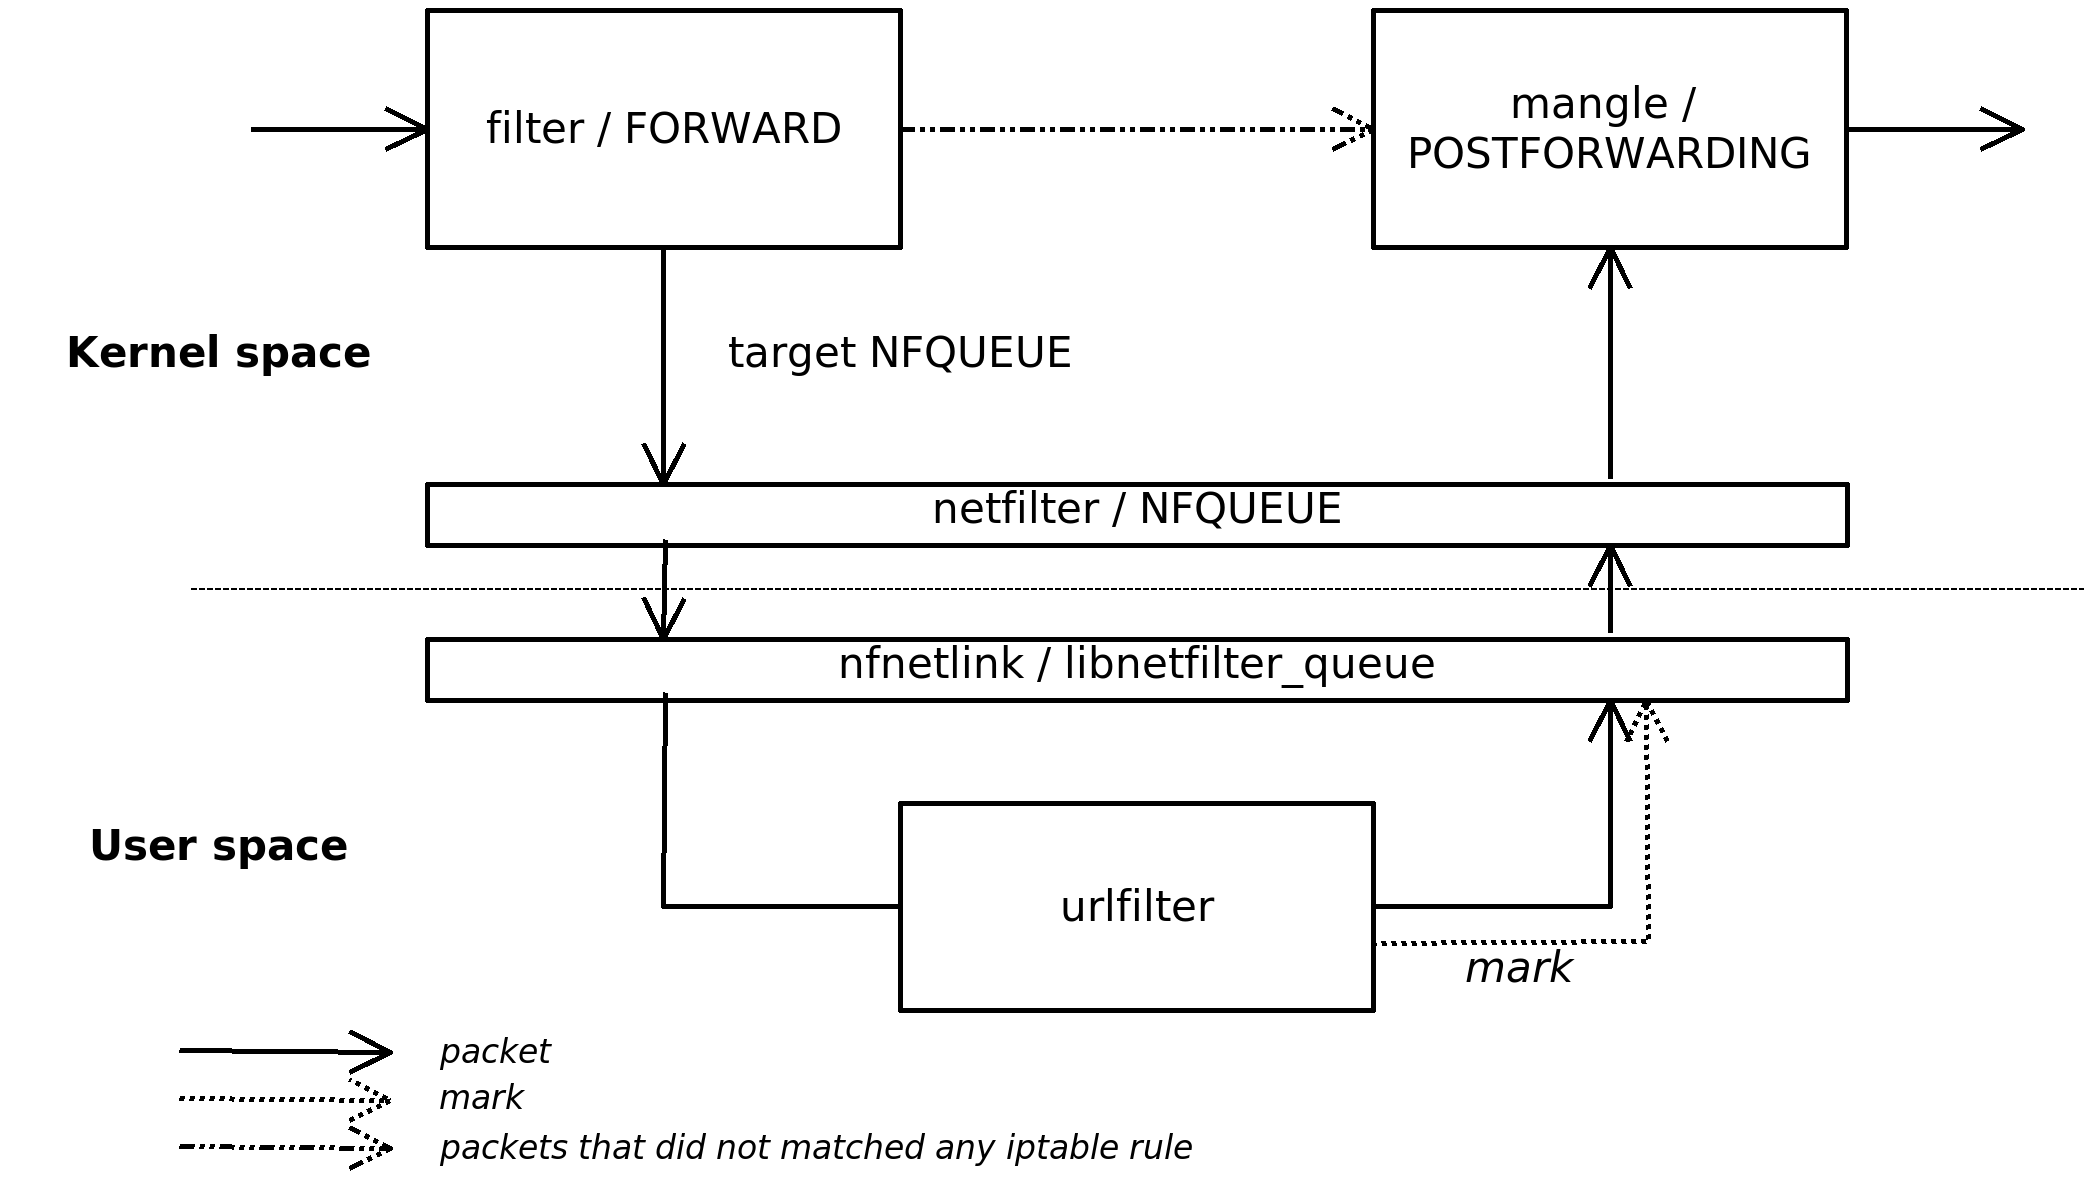
\includegraphics[scale=0.13]{pictures/schema1.png}
    \end{figure}
  \end{frame}

\newpage

\section{Implémentation}
\section<presentation>[Impl�mentation]{Impl�mentation}
  \begin{frame}
    \frametitle{Organisation du programme}
      Le programme contient :
      \begin{itemize}
        \item un \texttt{README} tr�s complet ;
        \item un r�pertoire base, regroupant plusieurs librairies externes (sous licences compatibles GPLv2) ;
        \item un fichier de configuration ;
        \item \texttt{queue.h/cc}, \texttt{packet.h/cc} et \texttt{conntrack.h/cc} qui r�alisent l'interception des paquets envoy�s �
        \texttt{NFQUEUE} (\texttt{queue.cc}), leur interpr�tation (\texttt{packet.cc}), et leur mise en relation avec un conntrack
        (\texttt{conntrack.cc}) ;
        \item \texttt{classifier.h/cc} qui sert � classer les paquets ;
        \item un fichier de base permettant le lancement des threads, un autre parsant le fichier de configuration et
        initialisant le classifier.
      \end{itemize}
  \end{frame}

  \begin{frame}
    \frametitle{Fonctionnement du logiciel}
      \begin{itemize}
        \item<1-> Regrouper les paquets appartenant � une m�me connexion, gr�ce � l'utilisation de
        \texttt{libnetfilter\_conntrack};
        \item<2-> D�terminer si le contenu de la connexion correspond � un protocole support�;
        \item<3-> Extraire la m�thode et l'url utilis�es par le client des paquets;
        \item<4-> Classifier et remonter l'information au noyau.
      \end{itemize}
  \end{frame}

  \begin{frame}
    \frametitle{Fonctionnement du logiciel}
      \begin{figure}[h]
        \centering
        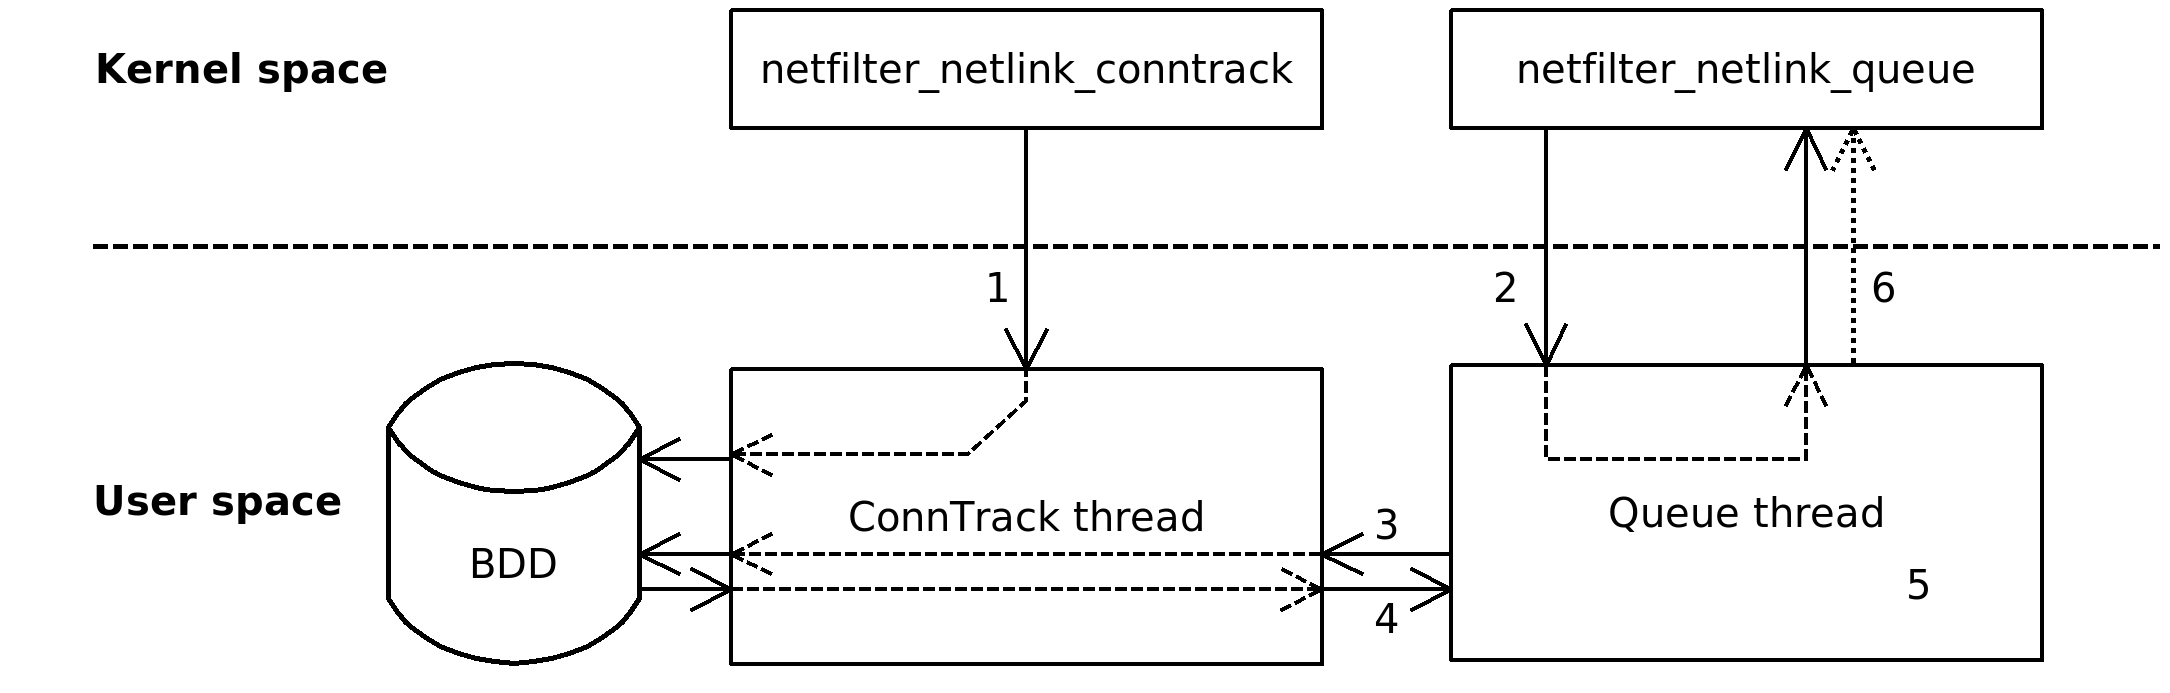
\includegraphics[width=\textwidth]{schema2.png}\\
        \title{Fonctionnement du module}
      \end{figure}
  \end{frame}

  \begin{frame}
    \frametitle{Fonctionnement pratique}
      \begin{itemize}
        \item<1-> Le 1\ier{} thread �coute sur un \texttt{netfilter\_netlink}, re�oit les mises � jour de la table conntrack du
        noyau et maintient une copie locale.
        \item<2-> Le 2\ieme{} thread intercepte les paquets arrivant sur une
        \texttt{NFQUEUE}, les parse, d�termine l'entr�e conntrack et r�cup�re l'objet \og Connection \fg{}
        correspondant, met � jour les deux buffers, puis appelle la m�thode \texttt{update} du classifier avant d'accepter le
        paquet, en le marquant.
        \item<3-> Le classifier surveille les buffers d'une connexion et prend une d�cision.
      \end{itemize}
  \end{frame}

  \begin{frame}
    \frametitle{Fiabilit� et limitation}
      \begin{itemize}
        \item<1-> Le protocole ftp est g�r� correctement.
        \item<2-> Les requ�tes en \emph{Keep-Alive} dans l'http ne sont pas g�r�es.
        \item<3-> L'application r�siste nativement aux attaques de types \emph{Denial of Service}.
      \end{itemize}
  \end{frame}

%\newpage

%\section*{Conclusion}
%\input{concl.tex}

\nocite{RW}
\nocite{C}
\nocite{S}

\newpage
\bibliography{biblio}{}
\bibliographystyle{amsalpha}
\addcontentsline{toc}{section}{\numberline{}Références}

\end{document}
